\documentclass[fleqn,answers]{exam}

%% Set page size and margins
\usepackage[a4paper,margin=2cm]{geometry}

\usepackage[utf8]{inputenc}
\usepackage[T1]{fontenc}
\usepackage{amsmath}
\usepackage{amssymb}
\usepackage{ctex}
\usepackage{graphicx}
\usepackage{multicol}
\usepackage{listings}
\setlength{\columnsep}{1pt}

%% Set code style
\definecolor{codegreen}{rgb}{0,0.6,0}
\definecolor{codegray}{rgb}{0.5,0.5,0.5}
\definecolor{codepurple}{rgb}{0.58,0,0.82}
\definecolor{backcolour}{rgb}{0.96,0.96,0.96}

\lstdefinestyle{mystyle}{
    backgroundcolor=\color{backcolour},
    commentstyle=\color{codegreen},
    keywordstyle=\color{magenta},
    numberstyle=\tiny\color{codegray},
    stringstyle=\color{codepurple},
    basicstyle=\ttfamily\footnotesize,
    breakatwhitespace=false,
    breaklines=true,
    captionpos=b,
    keepspaces=true,
    numbers=left,
    numbersep=5pt,
    showspaces=false,
    showstringspaces=false,
    showtabs=false,
    tabsize=2
}

\lstset{style=mystyle}

%% Set head & foot
\pagestyle{headandfoot}
\firstpageheadrule
\firstpageheader{西安交通大学}{大数据管理方法与应用}{课程作业}
\runningheader{西安交通大学}{大数据管理方法与应用}{课程作业}
\runningheadrule
\firstpagefooter{}{第\thepage\ 页(共\numpages 页)}{}
\runningfooter{}{第\thepage\ 页(共\numpages 页)}{}

\renewcommand{\solutiontitle}{\noindent\textbf{解:}\par\noindent}

\title{The Application of Expetation-Maximize Algorithm:\\ 3 Coins Problem and Gaussian Mixture Model}
\author{CanoY}

\begin{document}
\maketitle
\thispagestyle{headandfoot}
\begin{questions}
    \question{(a)推导三硬币模型的 EM 算法中隐变量后验分布的计算公式以及参数更新公式;\\
    (b)假设硬币 A、B、C 正面向上的概率分别是 0.7、0.3、0.6,按照三硬币模型的数据生成过程独立地重复 100 次试验并记录观测结果的序列;\\
    (c)利用 EM 算法根据上述观测序列估计各硬币正面向上的概率。}
    \question{参考《The Matrix Cookbook》推导高斯混合模型的 EM 算法中 M 步的参数
    更新公式。}
    \question{按下列参数生成高斯混合模型的数据,共有三个高斯混合成分,每个成分
    生成 300 个数据点。}
    \begin{align*}
        &\boldsymbol{\mu}_1=(3,1) &\Sigma_1=((1,-0.5);(-0.5,1))\\
        &\boldsymbol{\mu}_2=(8,10) &\Sigma_2=((2,0.8);(0.8,2))\\
        &\boldsymbol{\mu}_3=(12,2) &\Sigma_3=((1,0);(0,1))
    \end{align*}
使用 scikit-learn 库中的高斯混合模型实现上述数据的学习过程,
计算在不同个数的高斯混合成分下模型的 AIC 和 BIC 值,
并将学习得到的模型参数与真实模型参数进行对比。\\
~\\
1.(a)
\begin{solution}
        $$J(\theta,Q(z))=\sum\limits_i \sum\limits_{z_i} Q(z_i)\cdot\log(\frac{P(x_i,z_i \vert \theta)}{Q(z_i)}), \quad \theta=(\pi,p,q)$$
    \textbf{E step:}
    \begin{align*}
        Q^{t+1}(z)&=\arg\max\limits_{Q(z)} ~ J(\theta^t,Q(z))\\
        Q(z_i)&=P(z_i \vert x_i,\theta^t)\Leftarrow
            \begin{cases}
                \dfrac{P(x_i,z_i \vert \theta^t)}{Q(z_i)}=c,\\
                \sum\limits_{z_i} Q(z_i)=1
            \end{cases}\\
            &\begin{cases}
                P(z \vert x,\theta)&=\dfrac{P(x,z \vert \theta)}{P(x \vert \theta)}\\
                P(x,z \vert \theta)&=\pi^z p^x (1-p)^{1-x} + (1-\pi)^{1-z} q^x (1-q)^{1-x}\\
                P(x \vert \theta)&=P(x,z=1 \vert \theta)+P(x,z=0 \vert \theta)
            \end{cases}\\
        Q^{t+1}(z_i)&=P(z_i \vert x_i,\theta^t)\\
            &=\frac{
                (\pi^t)^{z_i} (p^t)^{x_i} (1-p^t)^{1-x_i} +
                (1-\pi^t)^{1-z_i} (q^t)^{x_i} (1-q^t)^{1-x_i}
            }
            {
                (\pi^t) (p^t)^{x_i} (1-p^t)^{1-x_i} +
                (1-\pi^t) (q^t)^{x_i} (1-q^t)^{1-x_i}
            }\\
        Q^{t+1}(z_i=1)&=\frac{(\pi^t) (p^t)^{x_i} (1-p^t)^{1-x_i}}
        {
            (\pi^t) (p^t)^{x_i} (1-p^t)^{1-x_i} +
            (1-\pi^t) (q^t)^{x_i} (1-q^t)^{1-x_i}
        }
    \end{align*}
    \textbf{M step:}
    \begin{align*}
        \theta^{t+1}&=\arg\max\limits_\theta ~ J(\theta,Q^{t+1}(z))\\
            &=\arg\max\limits_\theta ~ \sum\limits_i \sum\limits_{z_i} Q(z_i) \cdot \log(P(x_i,z_i \vert \theta))\\
        \textcircled{1}~
        \frac{\partial J(\theta,Q^{t+1}(z))}{\pi}&=\sum\limits_i \sum\limits_{z_i} \frac{Q^{t+1}(z_i)}{P(x_i,z_i \vert \theta)} \cdot \frac{\partial P(x_i,z_i \vert \theta)}{\partial \pi}\\
            &=\sum\limits_i [
                \frac{Q^{t+1}(z_i=1)}{\pi p^{x_i} (1-p)^{1-x_i}} \cdot p^{x_i} (1-p)^{1-x_i} -
                \frac{Q^{t+1}(z_i=0)}{(1-\pi) q^{x_i} (1-q)^{1-x_i}} \cdot q^{x_i} (1-q)^{1-x_i}
            ]\\
            &=\frac{1}{\pi} \sum\limits_i Q^{t+1}(z_i=1) - \frac{1}{1-\pi} \sum\limits_i Q^{t+1}(z_i=0)\\
        \frac{\partial J(\theta,Q^{t+1}(z))}{\pi}& \vert_{\pi=\pi^{t+1}}=0\\
        \pi^{t+1}&=\frac{\sum\limits_i Q^{t+1}(z_i=1)}{\sum\limits_i [Q^{t+1}(z_i=0)+Q^{t+1}(z_i=1)]}\\
            &=\frac{1}{n} \sum\limits_i Q^{t+1}(z_i=1)\\
        \textcircled{2}~
        \frac{\partial J(\theta,Q^{t+1}(z))}{p}&=\sum\limits_i \sum\limits_{z_i} \frac{Q^{t+1}(z_i)}{P(x_i,z_i \vert \theta)} \cdot \frac{\partial P(x_i,z_i \vert \theta)}{\partial p}\\
            &=\sum\limits_i
                \frac{Q^{t+1}(z_i=1)}{\pi p^{x_i} (1-p)^{1-x_i}} \cdot
                    [ \pi x_i p^{x_i-1} (1-p)^{1-x_i} - \pi p^{x_i} (1-x_i) (1-p)^{-x_i}]\\
            &=\sum\limits_i
                Q^{t+1}(z_i=1) (\frac{x_i}{p} - \frac{1-x_i}{1-p})\\
        \frac{\partial J(\theta,Q^{t+1}(z))}{p}& \vert_{p=p^{t+1}}=0\\
        p^{t+1}&=\frac{\sum\limits_i Q^{t+1}(z_i=1) x_i}{\sum\limits_i Q^{t+1}(z_i=1)}\\
        \textcircled{3}~
        \frac{\partial J(\theta,Q^{t+1}(z))}{q}&=\sum\limits_i \sum\limits_{z_i} \frac{Q^{t+1}(z_i)}{P(x_i,z_i \vert \theta)} \cdot \frac{\partial P(x_i,z_i \vert \theta)}{\partial q}\\
            \ &=\sum\limits_i
                Q^{t+1}(z_i=0) (\frac{x_i}{q} - \frac{1-x_i}{1-q})\\
        q^{t+1}&=\frac{\sum\limits_i Q^{t+1}(z_i=0) x_i}{\sum\limits_i Q^{t+1}(z_i=0)}\\
            &=\frac{\sum\limits_i (1-Q^{t+1}(z_i=1)) x_i}{\sum\limits_i (1-Q^{t+1}(z_i=1))}\\
    \end{align*}
    由推导过程可知, $\theta$中三个参数的更新都需要计算 $Q^{t+1}(z=1)$ ,提前计算有利于提高算法效率。
\end{solution}
\newpage
(b)生成的观测序列如图:
\begin{figure*}[!ht]
    \centering
    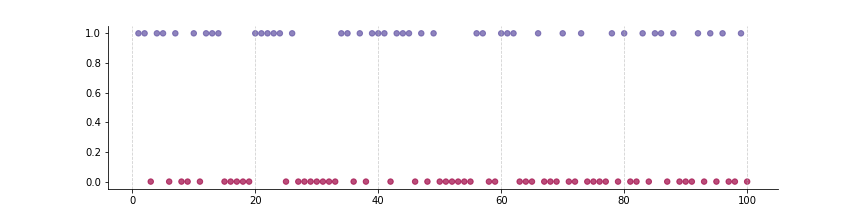
\includegraphics[width=18cm]{./figures/1b.png}
\end{figure*}\\
(c)预测结果如下:
\begin{table}[!ht]
    \centering
    \begin{tabular}{|c|ccc|c|}\hline
        &$\pi$&$p$&$q$&LL\\ \hline
        真实参数&0.700&0.300&0.600&-0.4943\\ \hline
        预测1& 0.248&0.776&0.329&-0.5798\\
        预测2& 0.598&0.440&0.440&-0.5798\\
        预测3& 0.047&0.760&0.424&-0.5798\\
        $\cdots$&&$\cdots$&&$\cdots$\\ \hline
    \end{tabular}
\end{table}\\
尽管有无穷多解,但它们的似然几乎相等。\\
~\\
2.
\begin{solution}
    $$J(\theta,Q(z))=\sum\limits_i \sum\limits_{z_i} Q(z_i)\cdot\log(\frac{P(\mathbf{x}_i,z_i \vert \theta)}{Q(z_i)}), \quad \theta=\{ \alpha_k,\boldsymbol{\mu}_k,\Sigma_k \}_{k=1}^K$$
\textbf{E step:}
\begin{align*}
    Q^{t+1}(z)&=\arg\max\limits_{Q(z)} ~ J(\theta^t,Q(z))\\
    Q^{t+1}(z_i)&=P(z_i \vert \mathbf{x}_i,\theta^t)\\
        &=\frac{P(\mathbf{x}_i \vert z_i,\theta^t)P(z_i \vert \theta^t)}
            {\sum\limits_{z_i} P(\mathbf{x}_i \vert z_i,\theta^t)P(z_i \vert \theta^t)}\\
    Q^{t+1}(z_i=k)&=\frac{\alpha_k P(\mathbf{x}_i \vert \boldsymbol{\mu}_k^t,\Sigma_k^t)}
    {\sum\limits_{k=1}^K \alpha_k P(\mathbf{x}_i \vert \boldsymbol{\mu}_k^t,\Sigma_k^t)}
\end{align*}
\textbf{M step:}
\begin{align*}
    \theta^{t+1}&=\arg\max\limits_\theta ~ J(\theta,Q^{t+1}(z))\\
        &=\arg\max\limits_\theta ~ \sum\limits_i \sum\limits_{z_i} Q(z_i) \cdot \log(P(\mathbf{x}_i,z_i \vert \theta))\\
    \textcircled{1}~
    L(\boldsymbol{\alpha},\nu)&=
        \sum\limits_i \sum\limits_{z_i} Q^{t+1}(z_i) \log P(\mathbf{x}_i,z_i \vert \theta) +
        \nu(\sum\limits_{k=1}^K \alpha_k -1)\\
    \frac{\partial L}{\partial \alpha_k}&=\sum\limits_i \frac{Q^{t+1}(z_i=k)}
        {\alpha_k P(\mathbf{x}_i \vert \boldsymbol{\mu}_k,\Sigma_k)} + \nu\\
        &=\sum\limits_i \frac{Q^{t+1}(z_i=k)}{\alpha_k} + \nu\\
        \frac{\partial L}{\partial \alpha_k}&\vert_{\alpha_k=\alpha_k^{t+1}}=0\\
        \sum\limits_i & \frac{Q^{t+1}(z_i=k)}{\alpha_k^{t+1}} + \nu=0\\
        \sum\limits_k \alpha_k^{t+1} &= \frac{\sum\limits_i \sum\limits_k Q^{t+1}(z_i=k)}{-\nu}\\
        &=\frac{m}{-\nu}=1\\
        \alpha_k^{t+1}&=\frac{1}{m}\sum\limits_i Q^{t+1}(z_i=k)\\
    \textcircled{2}~
    \log P(\mathbf{x}_i,z_i=k \vert \theta)&=\log \alpha_k\cdot P(\mathbf{x}_i\vert \boldsymbol{\mu}_k,\Sigma_k)\\
        &=\log\alpha_k -
            \frac{n}{2}\log 2\pi -
            \frac{1}{2}\log \vert \Sigma_k \vert - \\
            &\hspace{40pt} \frac{1}{2}(\mathbf{x}_i-\boldsymbol{\mu}_k)^T \Sigma_k^{-1} (\mathbf{x}_i-\boldsymbol{\mu}_k)\\
    \frac{\partial J(\theta,Q^{t+1}(z))}{\partial \boldsymbol{\mu}_k}&=-\sum\limits_i Q^{t+1}(z_i=k) \Sigma_k^{-1} (\mathbf{x}_i-\boldsymbol{\mu}_k)\\
    \frac{\partial J(\theta,Q^{t+1}(z))}{\partial \boldsymbol{\mu}_k}&\vert_{\boldsymbol{\mu}_k=\boldsymbol{\mu}_k^{t+1}}=0\\
    \boldsymbol{\mu}_k^{t+1}&=\frac{\sum\limits_i Q^{t+1}(z_i=k)\mathbf{x}_i}{\sum\limits_i Q^{t+1}(z_i=k)}\\
    \textcircled{3}~
    \frac{\partial J(\theta,Q^{t+1}(z))}{\partial \Sigma_k}\vert_{\Sigma_k=\Sigma_k^{t+1}}
        &=\frac{1}{2}\sum\limits_i Q^{t+1}(z_i=k) \cdot [-(\Sigma_k^{t+1})^{-1} + \\
            &\hspace{30pt} (\Sigma_k^{t+1})^{-1} (\mathbf{x}_i-\boldsymbol{\mu}_k) (\mathbf{x}_i-\boldsymbol{\mu}_k)^T (\Sigma_k^{t+1})^{-1}]=0\\
        &\sum\limits_i  Q^{t+1}(z_i=k) \cdot [\Sigma_k^{t+1} + (\mathbf{x}_i-\boldsymbol{\mu}_k) (\mathbf{x}_i-\boldsymbol{\mu}_k)^T]=0\\
        \Sigma_k^{t+1} &=\frac{
            \sum\limits_i Q^{t+1}(z_i=k) \cdot
            (\mathbf{x}_i-\boldsymbol{\mu}_k) (\mathbf{x}_i-\boldsymbol{\mu}_k)^T
            }
            {\sum\limits_i Q^{t+1}(z_i=k)}
\end{align*}
\end{solution}
\end{questions}
\newpage
3.\\
生成样本与高斯混合模型预测的分类结果如下:
\begin{figure*}[!ht]
    \centering
    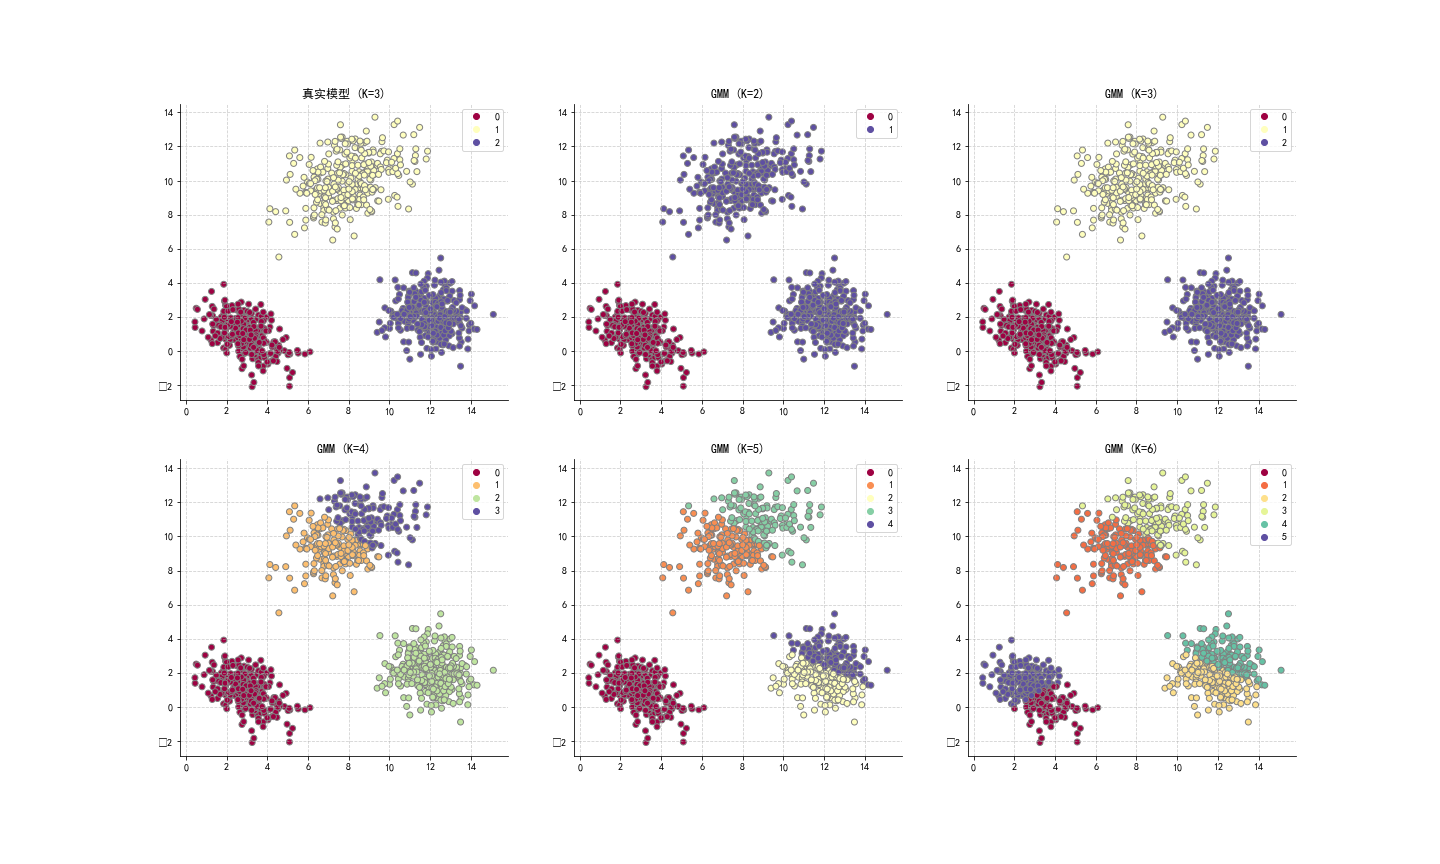
\includegraphics[width=18cm]{./figures/3.png}
\end{figure*}\\
AIC 和 BIC 值情况如下:
\begin{figure*}[!ht]
    \centering
    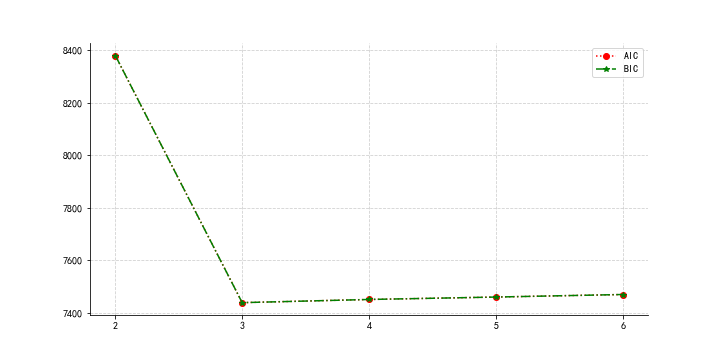
\includegraphics[width=18cm]{./figures/3_metrics.png}
\end{figure*}\\
\end{document}
